\documentclass[12pt,letterpaper]{article}
\usepackage{amsmath,amsthm,amsfonts,amssymb,amscd}
\usepackage{fullpage}
\usepackage{lastpage}
\usepackage{enumerate}
\usepackage{fancyhdr}
\usepackage{mathrsfs}
\usepackage[margin=3cm,bottom=6cm]{geometry}
\usepackage{wrapfig}
\usepackage{graphicx}

\setlength{\parindent}{0.0in}
\setlength{\parskip}{0.05in}

\renewcommand{\theenumi}{\bf\Alph{enumi}}


% Edit these as appropriate
\newcommand\course{Math 227C}
%\newcommand\semester{Spring 2019}     % <-- current semester
\newcommand\hwnum{1}                  % <-- homework number
\newcommand\yourname{Jun Allard} % <-- your name
%\newcommand\login{jcarberr}           % <-- your CS login

\newenvironment{answer}[1]{
  \subsubsection*{Problem \hwnum.#1}
}{\newpage}

\pagestyle{fancyplain}
\headheight 35pt
\lhead{ \course\ }
\chead{\textbf{ Problem Set 1 }}
%\rhead{Due {\bf Friday, April 13th}}
\headsep 20pt

\begin{document}


\begin{enumerate}

%%%%%%%%%%%%%% PROBLEM %%%%%%%%%%%%%%%%%%
\item Two fair dice are rolled, one after the other. 
\begin{enumerate}[i.]
\item Let $E_{6}$ be the event that the sum of the dice is 6. Let $F_4$ be the event that the first die is 4. Are these two events independent?
\item Let $E_{7}$ be the event that the sum of the dice is 7. Let $F_4$ be the event that the first die is 4. Are these two events independent?
\item Let $E_i$ be the event that the sum of the dice is $i$. Let $F_j$ be the event that the first die is $j$. For what values of $i$ and $j$ are these two events independent?
\end{enumerate}

%%%%%%%%%%%%%% PROBLEM %%%%%%%%%%%%%%%%%%
\item Suppose a cell signaling network has five components. Each component acts independently with probability $p_i$, $i=1,2,3,4,5$. These components form a signaling pathway shown in the diagram below. 
\begin{figure}[h!]
%\centering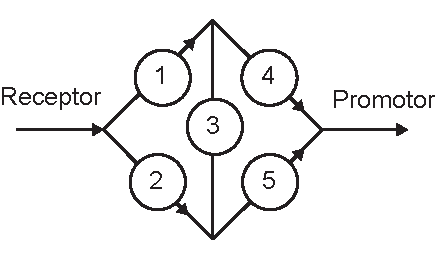
\includegraphics[width=8cm]{figP12.pdf}
\end{figure}
The system is said to work if a signal originating at the left end of the diagram (the receptor) can reach the right end (the promotor), where it can pass through a component only if that component is working. For instance, if components 1 and 4 both work, then the system works. Component 3 can transduce a signal in either direction (some \emph{scaffold proteins} in cells provide such multivalent functions). What is the probability that the system works? 

\end{enumerate}

\end{document}
